\chapter{Introducción} 
\label{chap:intro}
\comments{He visto que tienes un glosario, por ahora con pocos
  términos. Te interesa  utilizar glossaries de latex: https://es.sharelatex.com/learn/Glossaries}
\vspace{-0.2cm}

\lsection{Motivación del proyecto}

El derecho a la privacidad en Internet es algo que todo usuario
debería valorar y, por desgracia, el gran público no le da la
importancia que debería.
\comments{No es necesario que fuerces el salto de línea en latex:
  basta dejar una línea en blanco.}

\comments{Aquí faltan referencias. Conviene que reseñes que la
  privacidad hoy en día es un activo en sí, algo que debe cuidarse
  para garantizar derechos jurídicos y legales, pero también en pos de
  la gobernanaza digital. Esto último sólo es posible bajo el paraguas
  de tecnologías transparentes y de usuarios que hacen un uso
  consciente de esas tecnologías. En esta lid:
  \url{https://www.oecd.org/sti/ieconomy/oecdguidelinesontheprotectionofprivacyandtransborderflowsofpersonaldata.htm},
  \url{https://www.eugdpr.org/}. } No son pocas las noticias que están
apareciendo últimamente sobre empresas como Google relacionadas con la
invasión a la privacidad. Ésto, en gran parte, se ha visto
incrementado debido a la llegada de los \textit{smartphones} al
mercado(algo relativamente reciente, hace alrededor de 10 años). El
poder llevar en nuestro bolsillo todo un ordenador tiene el
inconveniente de que grandes empresas como las anteriormente
mencionadas pueden tener acceso a información en tiempo real de
nosotros, como por ejemplo a la hora a la que nos levantamos, la
localización de nuestra propia casa e incluso la ubicación real en
todo momento(y sí, de poco sirve deshabilitar la ubicación por GPS en
tu smartphone pues también la pueden averiguar mediante el inicio de
sesión en una red WiFi).  Por otro lado está el tema de las redes
sociales. Con el auge de Facebook, Instagram y Twitter, gran parte de
la población(en el caso de Norteamérica, casi dos terceras partes)
tiene perfil propio en la plataforma Facebook.

\begin{figure}[h]
	\centerline{
		\mbox{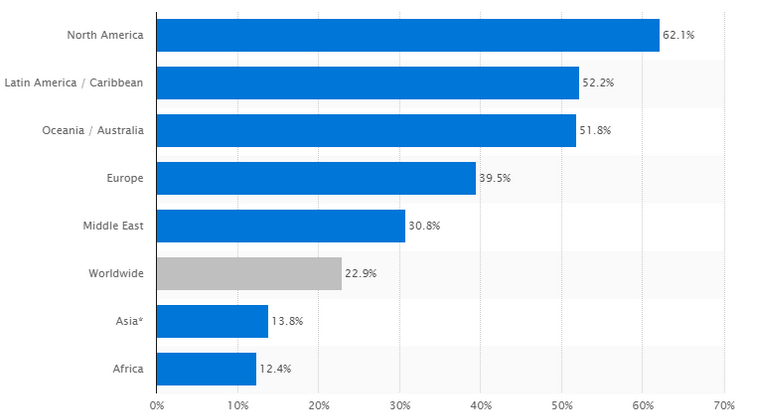
\includegraphics[width=4.00in]{images/sn.png}}
	}
	\caption{Porcentaje de población con perfil en Facebook}
	\label{fig:norm_Daugman}
\end{figure}

\commented{Esto}\comments{no olvides revisar la ortografía con un
  corrector automático} de por sí no es un dato negativo, el problema
viene cuando para realizar un registro en una página (como por
ejemplo, la web de un diario), la forma más sencilla es conectando con
tu perfil personal de Facebook. Ésto causa que, al interaccionar con
dicha página(ya sea publicando un comentario, o cualquier tipo de
actividad), te arriegues a que aparezca tu nombre real, con todo lo
que ello conlleva. Desde este punto, saber todo acerca de ese usuario
es tan sencillo como buscar en Google su nombre completo y entrar a su
perfil de Facebook, donde aparecen fotos, su dirección, entre otros.
En otros casos el iniciar sesión con la cuenta de Google ó Facebook
sirve para que dichas empresas conozcan mejor tus gustos y hobbies,
para así ofrecerte publicidad a medida.
\comments{Puedes añadir referencias, por ejemplo, a partir de los
  libros que te recomendé. Ahí tienes muchos ejemplos: haz uso de
  ellos. }

\commented{De aquí nace la verdadera motivación de este proyecto. La lucha contra
la privacidad en la red es algo que hemos ido perdiendo poco a poco,
pero mediante el uso de tecnologías para anonimizarse como las que
serán vistas en éste documento se pretende erradicar o, al menos,
mitigar éste problema.}\comments{Mira el comentario que figura más
abajo. Conviene que recalques lo que menciono allí: el objetivo es
doble. Por un lado, proporcionar un resumen de técnicas de protección
de la privacidad mediante anonimato. Por otro, saber identificar un
conjunto significativo de amenazas a la privacidad.}

Parte de la motivación también reside mi interés en el ámbito de la
seguridad informática \commented{que, desgraciadamente, no está demasiado
presente en el temario desarrollado en la carrera}\comments{di
simplemente que quieres profundizar en ello, pero vayas más allá: no
sabes quién va a estar en el tribunal, así que conviene evitar recelos
o suspicacias.}. Sin embargo, es un
tema de suma importancia y además sirve para poner en práctica
metodologías y lenguajes estudiados en el grado. \comments{Puedes
  poner alguna noticia sobre la demanda de expertos en
  ciberseguridad. Puedes encontrar muchas noticias sobre GDPR. }

En definitiva, el proyecto abarca un software modular compuesto de
varias herramientas funcionales por sí mismas y donde además el
requisito principal es la seguridad del
sistema(\textit{security-by-design}).  \comments{En esta caso, además
  y de forma quizás maś relevante privacy-by-design
  \cite{cavoukian2009privacy}. Ten en cuenta que esto se encuentra en
  la normativa GDPR europea que entra en vigor a partir de este mayo
  de 2018. Esto obliga a las empresas a ser muy cuidadosas en el
  tratamiento de PII (Personal Identifiable Information). Desde el
  punto de vista de un analista de seguridad, pues, es preciso contar
  con un conocimiento amplio de las posibles vulnerarciones y
  mecanismos de protección de la privacidad. Asimismo, y ante la
  posiblidad de  ser auditor de seguridad de sistemas, también se
  debe contar con una base sólida en técnicas de protección de
  privacidad. Conviene que esto quede bien claro, es muy importante. }
%bibliografía~\cite{article:Ejemplo}.


\lsection{Objetivos y enfoque}

Principalmente se pretenden lograr dos objetivos fundamentales en este proyecto.

El primero es el de hacernos conocedores más a fondo de las diferentes
vías a la hora de anonimizarnos en Internet, las variadas herramientas
que pretenden conseguir éste objetivo (así como las que pretenden
identificar a un usuario), las \commented{disparidades}\comments{Tal
  y como está resulta confuso. Conviene que te apoyes en textos como
  el Danezis \cite{danezis2010critical}: la privacidad se puede
  conseguir por diversas vías y, así, se tiene privacy as control,
  privacy as confidentiality y privacy as practice. Esto lo tienes
  referido en el libro de Nissenbaum \cite{lane2014privacy} mediante
  el marco BLT (Business-Legal-Technology). Si no me equivoco, te
  leíste el libro. Conviene que lo emplees y te apoyes en él para
  reforzar tu mensaje.} entre anonimato y
privacidad \modified{\ldots} En conclusión, realizar una investigación exhaustiva
sobre la privacidad en la red.

Por otro lado, y quizá el objetivo más importante, es el de poner en
práctica los conocimientos adquiridos en la investigación
anteriormente dicha. En este caso se ha diseñado, desarrollado y
probado una herramienta con numerosas y diversas funciones, cuyo
principal propósito es el de garantizarnos una experiencia lo más
anónima posible en todo momento.


\lsection{Metodología y plan de trabajo}

Éste documento se organiza de la siguiente manera:
\begin{itemize}
  \item Estado del Arte: El segundo capítulo explica todos y cada uno
    de los conceptos de los que trata este proyecto, es decir, el
    término privacidad, anonimato y la importancia de los mismos hoy
    en día. Además, se mostrarán ejemplos de herramientas y
    metodologías para anonimizarse.
  \item Análisis: El capítulo tres consta de la serie de requisitos,
    definidos según los objetivos deseados en las aplicaciones finales
    y delimitados por el alcance del proyecto.La funcionalidad de la
    herramienta desarrollada se resume tanto en el catálogo de
    requisitos como de casos de uso.
  \item Diseño: Este capítulo trata con detalle la fase de diseño,
    teniendo en cuenta la estructura de la aplicación y el flujo de
    navegación de la misma
  \item Desarrollo: En el quinto capítulo se encuentra explicado el
    método de desarrollo, las librerías utilizadas, los lenguajes en
    los que está programada la herramienta, las características
    Software del equipo de desarrollo y el porqué de dicha elección.
  \item Integración, pruebas y resultados: Aquí se tratan las pruebas
    unitarias realizadas, así como los resultados de las mismas y cómo
    se han integrado todos los módulos en la aplicación final.
  \item Conclusiones/Trabajo futuro: Por último, en este capítulo
    resumimos las conclusiones de la aplicación y el futuro trabajo
    que se requeriría para que la herramienta vaya creciendo.
\end{itemize}

\newpage \thispagestyle{empty} % Página vacía 
